% Template of basic phisics experiment 基于 article template，在此基础上做修改
% 设定文章编码类型，正文字号为五号则 zihao=5，正文字号为小四则 zihao=-4
\documentclass[zihao=5, UTF8]{article}		


% 自定义宏定义
\def\N{\mathbb{N}}
\def\F{\mathbb{F}}
\def\Z{\mathbb{Z}}
\def\Q{\mathbb{Q}}
\def\R{\mathbb{R}}
\def\C{\mathbb{C}}
\def\T{\mathbb{T}}
\def\S{\mathbb{S}}
\def\A{\mathbb{A}}
\def\I{\mathscr{I}}
\def\d{\mathrm{d}}
\def\p{\partial}


% 物理实验报告所需的其它宏包
\usepackage{ulem}   % \uline 下划线支持

% 导入基本宏包
\usepackage[UTF8]{ctex}     % 设置文档为中文语言
\usepackage[colorlinks, linkcolor=blue, anchorcolor=blue, citecolor=blue, urlcolor=blue]{hyperref}  % 宏包：自动生成超链接 (此宏包与标题中的数学环境冲突)
% \usepackage{docmute}    % 宏包：子文件导入时自动去除导言区，用于主/子文件的写作方式，\include{./51单片机笔记}即可。注：启用此宏包会导致.tex文件capacity受限。
\usepackage{amsmath}    % 宏包：数学公式
\usepackage{mathrsfs}   % 宏包：提供更多数学符号
\usepackage{amssymb}    % 宏包：提供更多数学符号
\usepackage{pifont}     % 宏包：提供了特殊符号和字体
\usepackage{extarrows}  % 宏包：更多箭头符号

% 列表环境设置
\usepackage{enumitem}   % 宏包：列表环境设置
    \setlist[enumerate]{itemsep=0pt, parsep=0pt, topsep=0pt, partopsep=0pt, leftmargin=3.5em} 
    \setlist[itemize]{itemsep=0pt, parsep=0pt, topsep=0pt, partopsep=0pt, leftmargin=3.5em}
    \newlist{circledenum}{enumerate}{1} % 创建一个新的枚举环境  
    \setlist[circledenum,1]{  
        label=\protect\circled{\arabic*}, % 使用 \arabic* 来获取当前枚举计数器的值，并用 \circled 包装它  
        ref=\arabic*, % 如果需要引用列表项，这将决定引用格式（这里仍然使用数字）
        itemsep=0pt, parsep=0pt, topsep=0pt, partopsep=0pt, leftmargin=3.5em
    }  
% 文章页面 margin 设置
\usepackage[a4paper]{geometry}  % 宏包：文章页面 margin 设置
    \geometry{top=0.75in}
    \geometry{bottom=0.75in}
    \geometry{left=0.75in}
    \geometry{right=0.75in}   % 设置上下左右页边距
    \geometry{marginparwidth=1.75cm}    % 设置边注距离（注释、标记等）

% 自定义数学环境
\usepackage{amsthm} % 宏包：数学环境配置
% theorem-line 环境自定义
    \newtheoremstyle{MyLineTheoremStyle}% <name>
        {11pt}% <space above>
        {11pt}% <space below>
        {}% <body font> 使用默认正文字体
        {}% <indent amount>
        {\bfseries}% <theorem head font> 设置标题项为加粗
        {：}% <punctuation after theorem head>
        {.5em}% <space after theorem head>
        {\textbf{#1}\thmnumber{#2}\ \ (\,\textbf{#3}\,)}% 设置标题内容顺序
    \theoremstyle{MyLineTheoremStyle} % 应用自定义的定理样式
    \newtheorem{LineTheorem}{Theorem.\,}
% theorem-block 环境自定义
    \newtheoremstyle{MyBlockTheoremStyle}% <name>
        {11pt}% <space above>
        {11pt}% <space below>
        {}% <body font> 使用默认正文字体
        {}% <indent amount>
        {\bfseries}% <theorem head font> 设置标题项为加粗
        {：\\ \indent}% <punctuation after theorem head>
        {.5em}% <space after theorem head>
        {\textbf{#1}\thmnumber{#2}\ \ (\,\textbf{#3}\,)}% 设置标题内容顺序
    \theoremstyle{MyBlockTheoremStyle} % 应用自定义的定理样式
    \newtheorem{BlockTheorem}[LineTheorem]{Theorem.\,} % 使用 LineTheorem 的计数器
% definition 环境自定义
    \newtheoremstyle{MySubsubsectionStyle}% <name>
        {11pt}% <space above>
        {11pt}% <space below>
        {}% <body font> 使用默认正文字体
        {}% <indent amount>
        {\bfseries}% <theorem head font> 设置标题项为加粗
        {：\\ \indent}% <punctuation after theorem head>
        {0pt}% <space after theorem head>
        {\textbf{#3}}% 设置标题内容顺序
    \theoremstyle{MySubsubsectionStyle} % 应用自定义的定理样式
    \newtheorem{definition}{}


% 有色文本框及其设置
\usepackage[dvipsnames,svgnames]{xcolor}    %设置插入的文本框颜色
\usepackage[strict]{changepage}     % 提供一个 adjustwidth 环境
\usepackage{framed}     % 实现方框效果
    \definecolor{graybox_color}{rgb}{0.95,0.95,0.96} % 文本框颜色。修改此行中的 rgb 数值即可改变方框纹颜色，具体颜色的rgb数值可以在网站https://colordrop.io/ 中获得。（截止目前的尝试还没有成功过，感觉单位不一样）（找到喜欢的颜色，点击下方的小眼睛，找到rgb值，复制修改即可）
    \newenvironment{graybox}{%
    \def\FrameCommand{%
    \hspace{1pt}%
    {\color{gray}\small \vrule width 2pt}%
    {\color{graybox_color}\vrule width 4pt}%
    \colorbox{graybox_color}%
    }%
    \MakeFramed{\advance\hsize-\width\FrameRestore}%
    \noindent\hspace{-4.55pt}% disable indenting first paragraph
    \begin{adjustwidth}{}{7pt}%
    \vspace{2pt}\vspace{2pt}%
    }
    {%
    \vspace{2pt}\end{adjustwidth}\endMakeFramed%
    }

% 各级标题自定义设置
\usepackage{titlesec}   
    % section标题自定义设置 
    \titleformat{\section}[hang]{\normalfont\huge\bfseries\centering}{第\,\thesection\,部分}{20pt}{}
    % subsection标题自定义设置 
    \titleformat{\subsection}[hang]{\normalfont\Large\bfseries}{\,\thesubsection\,}{8pt}{}
    % subsubsection标题自定义设置
    \titleformat{\subsubsection}[hang]{\normalfont\large\bfseries}{\,\thesubsubsection\,}{6pt}{}

% 外源代码插入设置
\usepackage{matlab-prettifier}
    \lstset{
        style=Matlab-editor,  % 继承matlab代码颜色等
    }
\usepackage[most]{tcolorbox} % 引入tcolorbox包 
\usepackage{listings} % 引入listings包
    \tcbuselibrary{listings, skins, breakable}
    \lstdefinestyle{matlabstyle}{
        language=Matlab,
        basicstyle=\small,
        breakatwhitespace=false,
        breaklines=true,
        captionpos=b,
        keepspaces=true,
        numbers=left,
        numbersep=15pt,
        showspaces=false,
        showstringspaces=false,
        showtabs=false,
        tabsize=2
    }
    \newtcblisting{matlablisting}{
        arc=0pt,
        top=0pt,
        bottom=0pt,
        left=1mm,
        listing only,
        listing style=matlabstyle,
        breakable,
        colback=white   % 选一个合适的颜色
    }

% table 支持
\usepackage{booktabs}   % 宏包：三线表
\usepackage{tabularray} % 宏包：表格排版
\usepackage{longtable}  % 宏包：长表格
\usepackage{tabularx}  % 宏包：宽表格
\usepackage{multirow}  % 宏包：表格中一格显示多个项目

% figure 设置
\usepackage{graphicx}  % 支持 jpg, png, eps, pdf 图片 
\usepackage{svg}       % 支持 svg 图片
    \svgsetup{
        % 指向 inkscape.exe 的路径
        inkscapeexe = C:/aa_MySame/inkscape/bin/inkscape.exe, 
        % 一定程度上修复导入后图片文字溢出几何图形的问题
        inkscapelatex = false                 
    }


% 图表进阶设置
\usepackage{float}     % 图表位置浮动设置 
\usepackage{caption}    % 图注、表注
    \captionsetup[figure]{name=图}  
    \captionsetup[table]{name=表}
    \captionsetup{labelfont=bf, font=small}

% 文章默认字体设置
    \usepackage{fontspec}   % 宏包：字体设置
       \setmainfont{SimSun}    % 设置中文字体为宋体字体
      \setCJKmainfont[AutoFakeBold=3]{SimSun} % 设置加粗字体为 SimSun 族，AutoFakeBold 可以调整字体粗细^     \setmainfont{Times New Roman} % 设置英文字体为Times New Roman


% 其它设置
    % equation 公式编号设置
        \makeatletter  
        \renewcommand{\theequation}{\thesection.\arabic{equation}}  
        \makeatother
    % 脚注设置
        \renewcommand\thefootnote{\ding{\numexpr171+\value{footnote}}}
    % 参考文献引用设置
        \bibliographystyle{unsrt}   % 设置参考文献引用格式为unsrt
        \newcommand{\upcite}[1]{\textsuperscript{\cite{#1}}}     % 自定义上角标式引用
    % 文章序言设置
        \newcommand{\cnabstractname}{序言}
        \newenvironment{cnabstract}{%
            \par\Large
            \noindent\mbox{}\hfill{\bfseries \cnabstractname}\hfill\mbox{}\par
            \vskip 2.5ex
            }{\par\vskip 2.5ex}


% 页眉页脚设置
\usepackage{fancyhdr}   %宏包：页眉页脚设置
    \pagestyle{fancy}
    \fancyhf{}
    \cfoot{\thepage}
    \renewcommand\headrulewidth{1pt}
    \renewcommand\footrulewidth{0pt}
    \rhead{\bfseries 分组序号: YK04-2}    
    \chead{《基础物理实验》实验报告,\ 韩初晓,\ 2023K8009908002}
    \lhead{2024.10.10}

% 文档信息设置
%\title{这里是标题\\The Title of the Report}
%\author{丁毅\\ \footnotesize 中国科学院大学，北京 100049\\ Yi Ding \\ %\footnotesize University of Chinese Academy of Sciences, Beijing %100049, China}
%\date{\footnotesize 2024.8 -- 2025.1}

% 开始编辑文章

\begin{document}
\noindent\begin{flushright}
    \zihao{2}{分组序号: YK04-2}
\end{flushright}

\setCJKfamilyfont{boldsong}[AutoFakeBold = {2.17}]{SimSun}
\newcommand*{\boldsong}{\CJKfamily{boldsong}}


\begin{center}\large
    \noindent{\Huge\bfseries\boldsong《基础物理实验》实验报告 }
    \\\vspace{0.4cm}
    \noindent\textit{
        \textbf{\boldsong 实验名称：}\uline{\hspace{0.3cm} 气轨上弹簧振子的简谐振动及瞬时速度的测定\hspace{0.3cm}}\hspace{0.4cm} 
        指导教师：\uline{\hspace{1.0cm}姚楚豪\hspace{1.0cm}}}
    \\\vspace{0.1cm}
    \noindent\textit{
        姓名：\uline{\,\,\,韩初晓\,\,\,}\hspace{0.2cm}
        学号：\uline{\,\,\,{\upshape 2023K8009908002}\,\,\,}\hspace{0.2cm}
        专业：\uline{\,\,\,计算机科学与技术\,\,\,}\hspace{0.2cm}
        班级：\uline{\,\,\,\upshape{2306}\,\,\,}}
    \\\vspace{0.1cm}
    \noindent\textit{
        实验日期：\uline{\,\,{\upshape 2024.10.10}\,\,}\hspace{0.2cm}
        实验地点：\uline{\,\,\,教学楼{\upshape716}\,\,\,}\hspace{0.2cm}
        是否调课/补课：\uline{\hspace{0.5cm}否\hspace{0.5cm}}\hspace{0.2cm}
        成绩：\uline{\hspace{2cm}}}
\end{center}
% \vspace{-0.2cm}
\noindent\rule{\textwidth}{0.1em}   % 分割线

% 控制目录不换页
\vspace{1cm}
\setcounter{tocdepth}{2}  % 目录深度为 2（不显示 subsubsection）
\noindent\begin{minipage}{\textwidth}\centering
\tableofcontents\thispagestyle{fancy}   % 显示页码、页眉等   
\end{minipage}  
\newpage

\section{实验目的}\thispagestyle{fancy} 

\begin{enumerate}
    \item 观察简谐振动现象，测定简谐振动的周期。
    \item 求弹簧的倔强系数 $\bar{k}$ 和有效质量 $\overline{m_0}$。
    \item 观察简谐振动的运动学特征。
    \item 验证机械能守恒定律。
    \item 用极限法测定瞬时速度。
    \item 深入了解平均速度和瞬时速度的关系。
\end{enumerate}

\section{实验用具}

\begin{figure}[H]
    \centering
    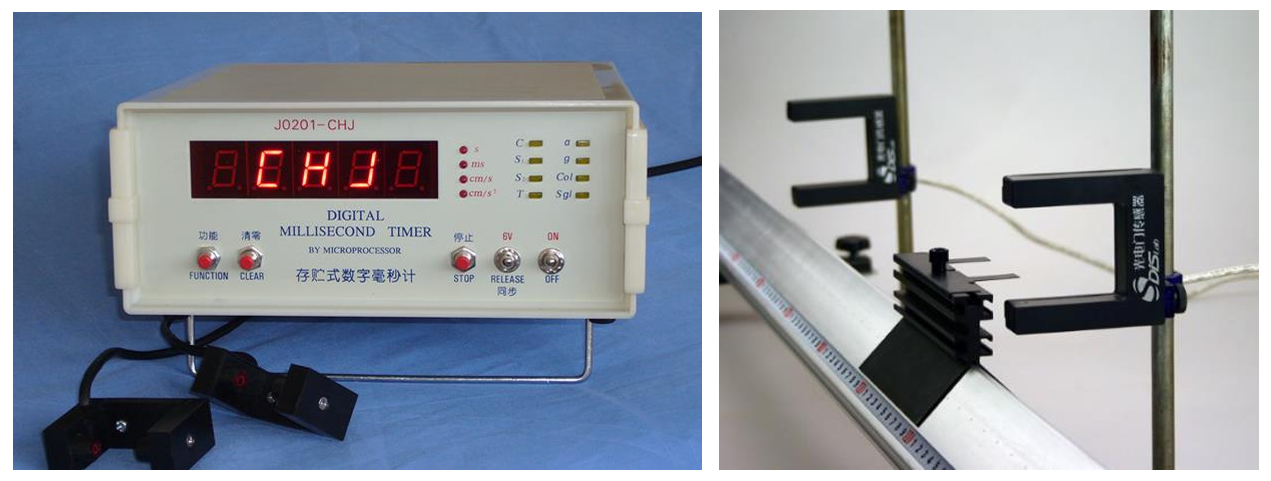
\includegraphics[width=0.8\textwidth]{./数字毫秒计和光电门传感器.png}
    \caption{数字毫秒计和光电门传感器}
    \label{fig:数字毫秒计和光电门传感器}
\end{figure}

\begin{figure}[H]
    \centering
    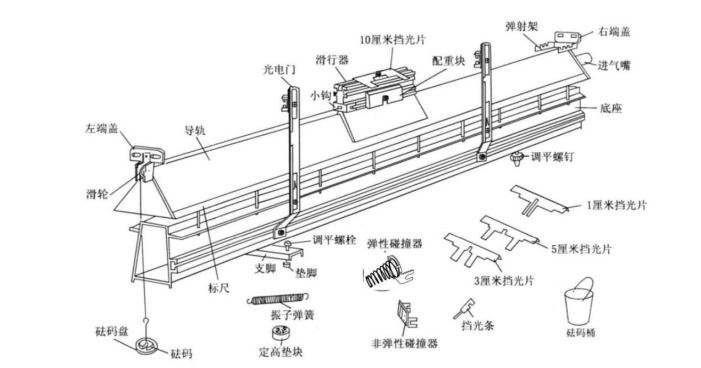
\includegraphics[width=0.8\textwidth]{./气垫导轨示意图部件.png}
    \caption{气垫导轨示意图部件}
    \label{fig:气垫导轨示意图部件}
\end{figure}

\begin{longtable}{|c|c|}
\hline
\textbf{实验用具} & \textbf{用途} \\
\hline
\endfirsthead
\hline
\textbf{实验用具} & \textbf{用途} \\
\hline
\endhead
\hline
\endfoot

气垫导轨 & 提供一个无摩擦的环境，减少阻力，确保滑块的简谐运动。 \\
滑块 & 作为实验的主要运动体，用于观察简谐振动。 \\
附加砝码 & 改变系统的质量，从而影响简谐振动的周期。 \\
弹簧 & 产生恢复力，使滑块发生简谐振动。 \\
U型挡光片 & 用于测量速度，通过遮挡光源来监测滑块的位置变化。 \\
平板挡光片 & 用于测量周期，通过光电传感器检测滑块通过周期性的运动。 \\
数字毫秒计 & 精确测量时间，记录振动的周期和速度。 \\
天平 & 用于测量附加砝码的质量，确保实验数据的准确性。 \\
\end{longtable}

\section{实验原理}

\subsection{弹簧振子简谐振动的原理}

在气垫导轨上，滑块与两弹簧连接，滑块做简谐振动。假设滑块质量为 $m_1$，处于平衡位置时，弹簧的伸长量为 $x_0$。当滑块位移为 $x$ 时，弹簧分别施加的力为 $-k_1(x + x_0)$ 和 $-k_1(x - x_0)$，其中 $k_1$ 是弹簧的劲度系数。由牛顿第二定律，得运动方程：

\[
m_1 \ddot{x} = -k(x)
\]

其中 $k = 2k_1$。此方程的解为：

\[
x(t) = A \sin(\omega_0 t + \varphi_0)
\]

其中 $A$ 为振幅，$\omega_0 = \sqrt{k/m}$ 为固有频率。

\subsubsection{振动周期与质量关系}

振动系统的有效质量为 $m = m_0 + m_1$，其中 $m_0$ 是弹簧的有效质量，$m_1$ 为滑块质量。振动周期 $T$ 与 $\omega_0$ 的关系为：

\[
T = 2\pi \sqrt{\frac{m}{k}} = 2\pi \sqrt{\frac{m_1 + m_0}{k}}
\]

平方后得：

\[
T^2 = \frac{4\pi^2 (m_1 + m_0)}{k}
\]

通过改变 $m_1$，测得不同 $T$ 值，并绘制 $T^2$ 与 $m_1$ 的关系曲线，斜率为 $\frac{4\pi^2}{k}$，可以计算出 $k$ 的值，截距得到 $m_0$。

\subsection{运动学特征与能量分析}

\subsubsection{速度与位置关系}

对振动方程求导，得到瞬时速度：

\[
v(t) = A \omega_0 \cos(\omega_0 t + \varphi_0)
\]

速度与位置满足关系：

\[
v^2 = \omega_0^2 (A^2 - x^2)
\]

当 $x = A$ 时，$v = 0$；当 $x = 0$ 时，$v = \pm A \omega_0$，此时速度最大。

\subsubsection{机械能守恒}

在任何时刻，系统的动能和势能分别为：

\[
E_k = \frac{1}{2} (m_1 + m_0) v^2, \quad E_p = \frac{1}{2} k x^2
\]

系统的总机械能 $E$ 为：

\[
E = E_k + E_p = \frac{1}{2} k A^2
\]

由于总能量守恒，系统的机械能在振动过程中保持不变。

\subsection{瞬时速度的测定}

瞬时速度是物体在某一时刻的速度，理论定义为：

\[
v_{\text{瞬}} = \lim_{\Delta t \to 0} \frac{\Delta s}{\Delta t}
\]

实验中，通过测量小时间间隔内的平均速度来间接测定瞬时速度。假设滑块从 A 点下滑，经过距离 $\Delta s$，时间为 $\Delta t$，其平均速度为：

\[
v = \frac{\Delta s}{\Delta t}
\]

当 $\Delta t \to 0$ 时，平均速度的极限值即为瞬时速度 $v_0$。实验中通过改变挡光距离 $\Delta s$，测量不同时间间隔内的平均速度，并绘制 $v$ 与 $\Delta t$ 的图线，外推至 $\Delta t = 0$ 处，得到瞬时速度。


\section{实验内容}

1. 学会使用光电门测量滑块的速度，并使用它来测量振动周期。

2. 调节气垫导轨至水平状态，测量滑块在任意两点的速度变化，验证气垫导轨是否水平。

3. 分别取振幅 $A = 10.0, 20.0, 30.0, 40.0$ cm，测量相应的振动周期，分析周期与振幅的关系。

4. 在滑块上加骑码（铁片），固定振幅 $A = 40.0$ cm，增加骑码测量周期 $T$。绘制 $T^2$ 对质量 $m$ 的图，求得弹簧劲度系数 $k$ 和有效质量 $m_0$。

5. 安装 U 型挡光片，测量速度，绘制 $v^2$ 对 $x^2$ 的图，进行拟合，求得斜率和截距，验证 $- \omega_0^2$ 与 $A^2 \omega_0^2$ 是否为斜率和截距。

6. 固定振幅 $A = 40.0$ cm，测量不同位置 $x$ 处的速度，计算动能与势能，并比较各位置的机械能，验证机械能是否守恒。

7. 改变挡光片距离，测量滑块从静止下滑时的平均速度，绘制 $v$ 对 $\Delta t$ 和 $\Delta s$ 的图，使用外推法求瞬时速度。

8. 改变气轨的倾斜角度 $\theta$，重复上述实验。

9. 改变 $A$ 点到 $P$ 点的距离 $l$（设置为 $60$ cm），重复实验。

\section{数据整理与计算}

\subsection{实验仪器的调试}
\begin{table}[H]
  \centering
	\begin{tabular}{|l|l|l|}
		\hline
		$V_1(cm/s)$  & $V_2(cm/s)$  & 误差(\%)          \\ \hline
		27.65 & 27.53 & 0.4 \\ \hline
		26.32 & 26.41 & 0.3 \\ \hline
		25.49 & 25.50  & 0.03  \\ \hline
	\end{tabular}
\end{table}

\subsection{测量弹簧振子的振动周期并考察振动周期和振幅的关系}
滑块的振幅$A$分别取10cm, 20cm, 30cm, 40cm，测得的振动周期如下：
\begin{table}[H]
  \centering
	\begin{tabular}{|l|l|l|l|l|}
		\hline
		& 10cm     & 20cm     & 30cm     & 40cm    \\ \hline
		T1(ms) & 1572.77  & 1569.69  & 1569.18  & 1568.02 \\ \hline
		T2(ms) & 1572.91  & 1570.00  & 1568.88  & 1568.21 \\ \hline
		T3(ms) & 1574.27  & 1569.88  & 1569.29  & 1568.31  \\ \hline
		T4(ms) & 1575.03  & 1569.95  & 1569.25  & 1568.51 \\ \hline
		T5(ms) & 1575.40  & 1570.06  & 1569.42  & 1568.55 \\ \hline
		T      & 1574.076 & 1569.916 & 1569.204 & 1568.395 \\ \hline
	\end{tabular}
  \caption{不同振幅下的振动周期}
  \label{tab:不同振幅下的振动周期}
\end{table}

根据以上图表，利用Python在两种不同的坐标尺度下绘制T-A关系曲线，结果如下：

\begin{figure}[H]
    \centering
    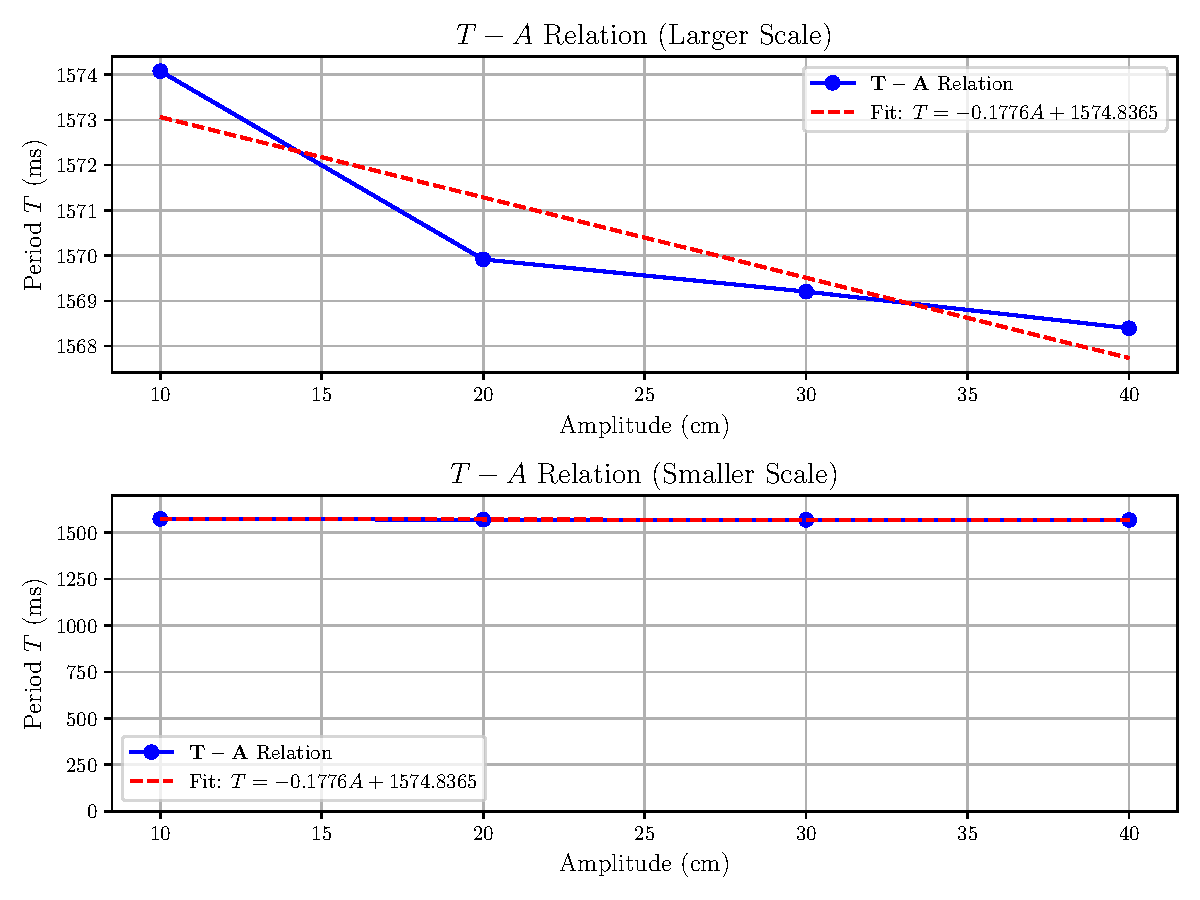
\includegraphics[width=0.8\textwidth]{./t_vs_a.pdf}
    \caption{振动周期与振幅的关系}
    \label{fig:振动周期与振幅的关系}
\end{figure}

由图像可知，改变振幅后周期无明显变化。因此，基本上可以认为，在实验误差允许的范围内，验证了理论推
导部分所认为的“简谐运动周期与振幅无关”这一结论。

\subsection{测量弹簧振子的振动周期并考察振动周期和质量的关系}
在滑块上加骑码（铁片）。对一个确定的振幅（$A = 40.0 \text{cm}$）每增加一个骑码测量一组$T$。(骑码不能加太多，以阻尼不明显为限。)作$T^2 - m$的图，如果$T$与$m$的关系式如公式\eqref{eq:Tm}所示，则$T^2 - m$ 的图应为一条直线，其斜率为$4\pi^2/k$，截距为$4\pi^2 m_0/k$ 。用最小二乘法做直线拟合，求出$k$和$m_0$。

\begin{table}[H]
  \centering
	\begin{tabular}{|l|l|l|l|l|l|}
		\hline
		& 1        & 2        & 3        & 4        & 5        \\ \hline
		T1(ms)  & 1570.25  & 1614.73  & 1656.67  & 1697.89  & 1738.67  \\ \hline
		T2(ms)  & 1570.55  & 1614.63  & 1657.13  & 1698.30  & 1738.91  \\ \hline
		T3(ms)  & 1570.55  & 1614.58  & 1657.19  & 1698.40  & 1738.97   \\ \hline
		T4(ms)  & 1570.72   & 1614.81  & 1657.40  & 1698.45  & 1738.71  \\ \hline
		T5(ms)  & 1570.96   & 1614.79  & 1657.24  & 1698.53  & 1739.20  \\ \hline
		T6(ms)  & 1571.01  & 1614.84  & 1657.72  & 1698.44  & 1739.02  \\ \hline
		T7(ms)  & 1571.15  & 1614.98  & 1657.62  & 1698.31  & 1739.33  \\ \hline
		T8(ms)  & 1571.17  & 1614.66  & 1657.67  & 1698.49  & 1739.20  \\ \hline
		T9(ms)  & 1571.08  & 1615.10  & 1657.48  & 1698.42  & 1739.11  \\ \hline
		T10(ms) & 1571.00  & 1614.66  & 1657.23  & 1698.65  & 1739.15  \\ \hline
		T       & 1570.844 & 1614.778 & 1657.335 & 1698.388 & 1739.027 \\ \hline
		m(g)    & 217.12   & 229.48   & 241.95   & 251.69   & 264.23   \\ \hline
	\end{tabular}
  \caption{不同质量下的振动周期}
  \label{tab:不同质量下的振动周期}
\end{table}

根据以上数据，绘制$T^2 - m$的图像，结果如下：

\begin{figure}[H]
    \centering
    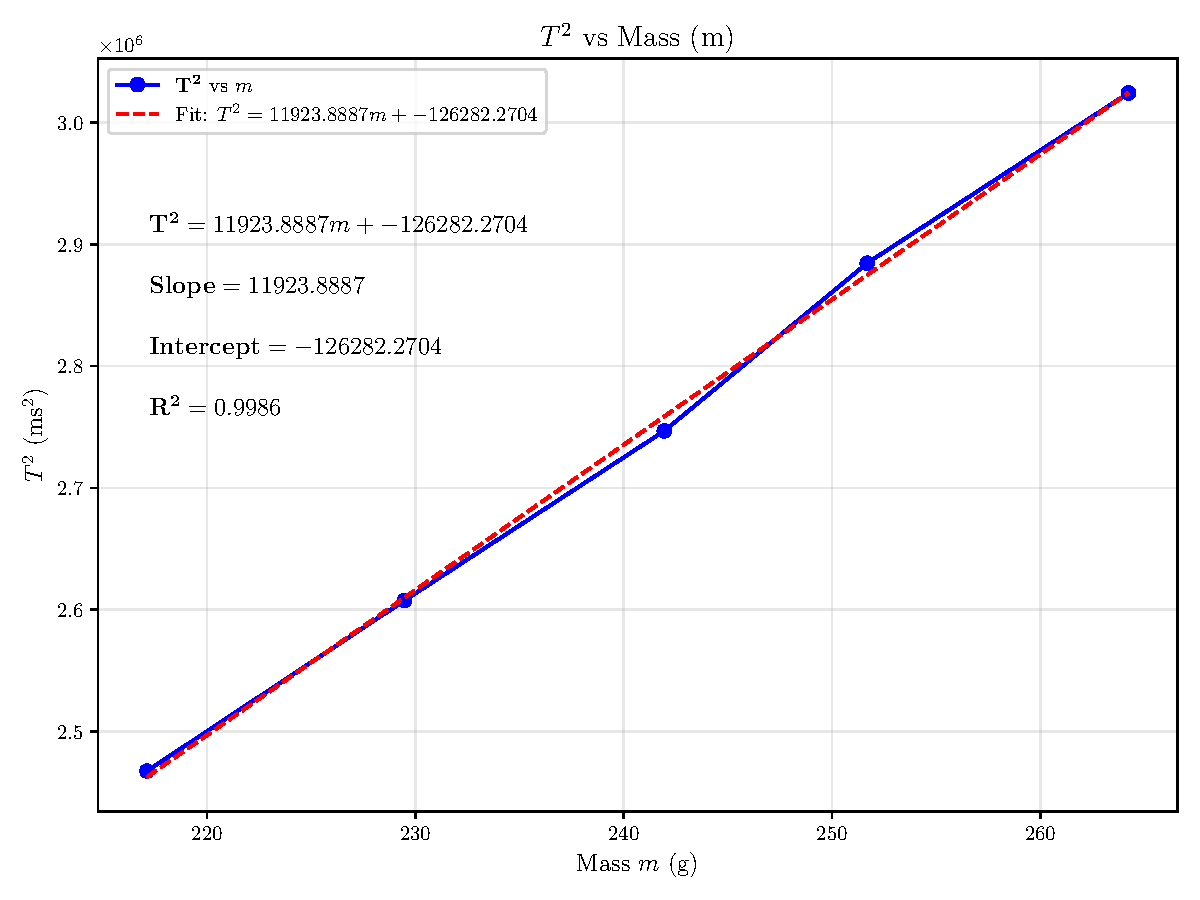
\includegraphics[width=0.8\textwidth]{./t2_vs_m.pdf}
    \caption{振动周期平方与质量的关系}
    \label{fig:振动周期平方与质量的关系}
\end{figure}

从图像可以看出，线性拟合的情况非常理想，实际图像与线性拟合的曲线几乎重合。斜率 $K = 11923.8887 = \frac{4 \pi^2}{k}$，因此劲度系数 $k = 3.311 \, \text{N/m}$，弹簧的有效质量 $m_0 = -10.591 \, \text{g}$。

\subsection{测量弹簧振子的速度与位移关系}

在滑块上装上U型挡光片，可测量速度。作$v^2 - x^2$的图，看该图是否为一条直线，并进行直线拟合，看斜率是否为$-\omega_0^2$，截距是否为$A^2\omega_0^2$，其中$\omega_0 = \frac{2\pi}{T}$，$T$可测出。固定振幅$A = 40.0$ cm，测量不同位置$x$处的速度如下表所示。

\begin{table}[H]
  \centering
	\begin{tabular}{|l|l|l|l|l|l|}
		\hline
		& 10cm        & 15cm   & 20cm        & 25cm        & 30cm        \\ \hline
		V1(cm/s) & 143.06      & 141.17 & 129.87      & 116.60       & 94.83      \\ \hline
		V2(cm/s) & 144.93      & 140.06 & 127.90      & 117.37      & 94.61      \\ \hline
		V3(cm/s) & 143.68      & 138.70 & 129.20      & 114.97      & 90.63      \\ \hline
		V(cm/s)  & 143.890 & 139.977 & 128.99 & 116.313 & 93.357 \\ \hline
	\end{tabular}
  \caption{不同位置下的速度}
  \label{tab:不同位置下的速度}
\end{table}

根据上述表格，绘制$v^2 - x^2$的图像，结果如下：

\begin{figure}[H]
    \centering
    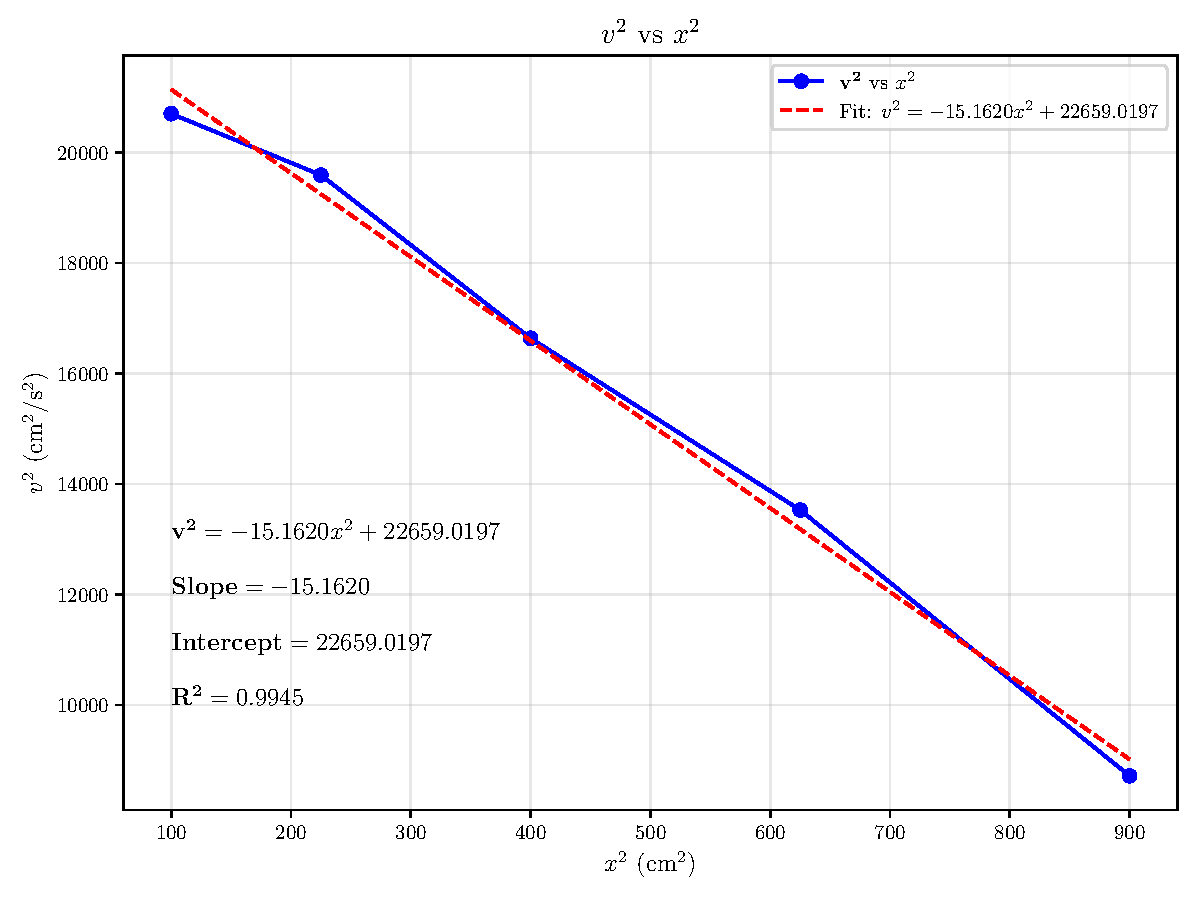
\includegraphics[width=0.8\textwidth]{./v2_vs_x2.pdf}
    \caption{速度平方与位移平方的关系}
    \label{fig:速度平方与位移平方的关系}
\end{figure}

根据理论推导，$v^2 - x^2$的图像应为一条直线，斜率为$-\omega_0^2$，截距为$A^2\omega_0^2$。从图像可以看出，线性拟合的情况非常理想，实际图像与线性拟合的曲线几乎重合。斜率 $K = -15.1620 = -\omega_0^2$，截距 $B = 22659.0197 = A^2\omega_0^2$，因此$\omega_0 = 3.893 \text{s}^{-1}$，$T = \frac{2\pi}{\omega_0} = 1.614 \text{s}$。这个周期数据与上一个实验测得的结果$1.571 \text{s}$相比，误差为$2.7\%$。根据前面的测量结果，$A = 0.4 \text{m}$，因此$A^2\omega_0^2 = 25.6 \text{m}^2/\text{s}^2$，与本实验测得的结果相比，误差为$11.8\%$。

\subsection{验证弹簧振子的机械能守恒}

固定振幅（如取$A = 40.0\text{cm}$），测出不同 $x$处的滑块速度，由此算出振动过程中经过每一个$x$的动能和势能，并对各$x$处的机械能进行比较，得出结论。根据前文的计算结果，弹簧的劲度系数 $k = 3.311 \text{N/m}$，有效质量 $m_0 = -10.591 \text{g}$，因此系统的有效质量为 $m = m_1 + m_0 = 0.21712 - 0.010591 = 0.206529 \text{kg}$。根据公式$E_k = \frac{1}{2} m v^2$和$E_p = \frac{1}{2} k x^2$，可以计算出各个位置的动能和势能，结果如下：
\begin{table}[H]
  \centering
	\begin{tabular}{|l|l|l|l|l|l|}
		\hline
		\textbf{x (cm)} & \textbf{10} & \textbf{15} & \textbf{20} & \textbf{25} & \textbf{30} \\ \hline
		\textbf{V (cm/s)} & 143.89 & 139.977 & 128.99 & 116.313 & 93.357 \\ \hline
		\textbf{Ek (J)} & 0.2138 & 0.2023 & 0.1718 & 0.1397 & 0.0900 \\ \hline
		\textbf{Ep (J)} & 0.0166 & 0.0372 & 0.0662 & 0.1035 & 0.1490 \\ \hline
		\textbf{E (J)} & 0.2304 & 0.2396 & 0.2380 & 0.2432 & 0.2390 \\ \hline
		\textbf{相对误差 (\%)} & 3.223 & 0.652 & 0.003 & 2.161 & 0.406 \\ \hline
	\end{tabular}
\end{table}

根据上述表格，绘制$x-E$的图像，结果如下：

\begin{figure}[H]
    \centering
    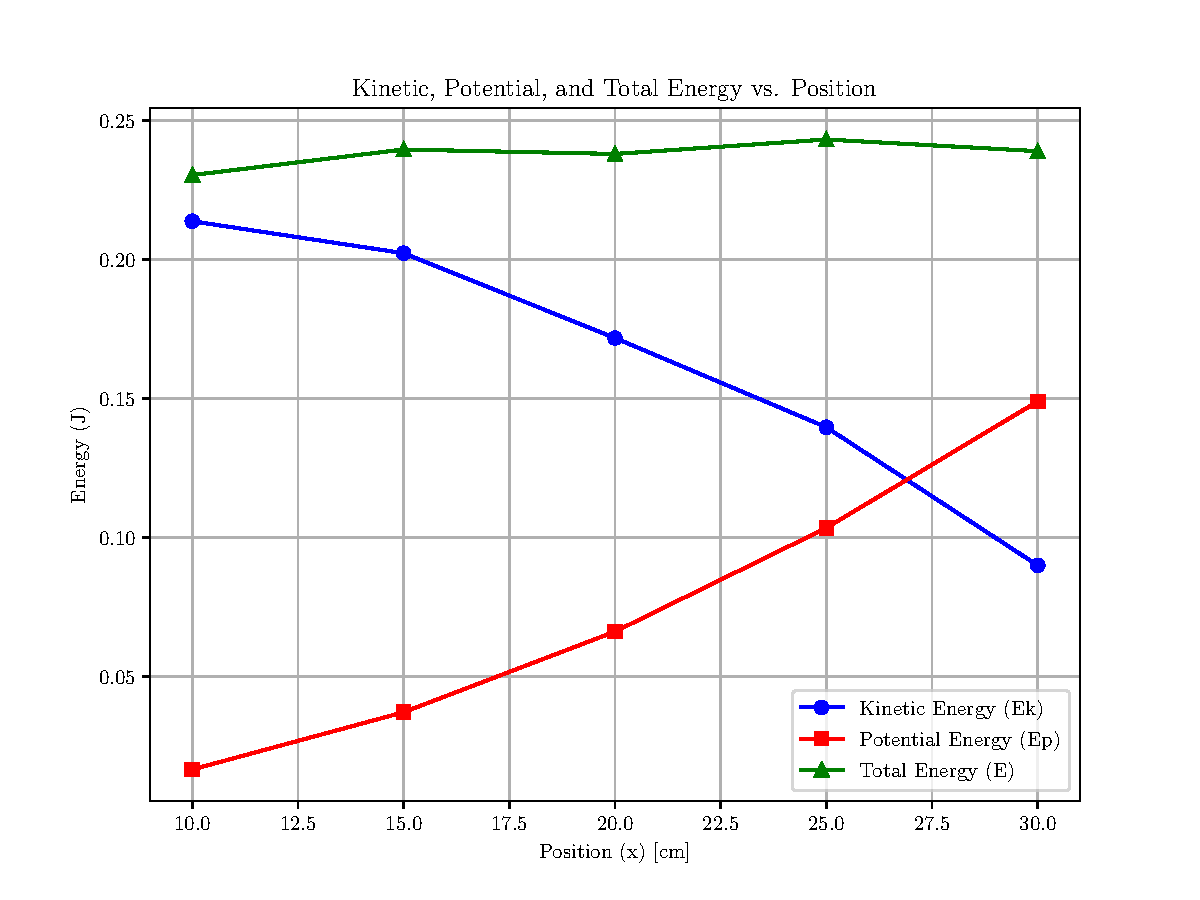
\includegraphics[width=0.8\textwidth]{./e_const.pdf}
    \caption{验证机械能守恒定律}
    \label{fig:验证机械能守恒定律}
\end{figure}

由图可知，动能和势能在该区间内有较大的变化，但二者之和，即机械能则几乎不变，在误差允许范围内,在振动过程中算出的总机械能大致是不变的，其相对于平均值的偏离均在$\pm 3.3\%$以内，在误差允许范围内,可以认为该实验的结论支持机械能守恒定律的正确性。

\subsection{改变弹簧振子的振幅$A$，由$V_{max}^2-A^2$关系求k}

改变弹簧振子的振幅$A$，测相应的$V_{max}$，由$V_{max}^2 - A^2$关系求$k$，与实验内容3的结果进行比较
将光电门固定在平衡位置，拉动滑块至不同的$A$处，从静止开始释放，测量其在经过平衡位置时的速度，即为该振幅$A$对应的最大速度$v_{max}$
\begin{table}[H]
  \centering
	\begin{tabular}{|l|l|l|l|l|l|}
		\hline
		& 10    & 15          & 20    & 25          & 30    \\ \hline
		Vmax1(cm/s) & 39.42 & 57.54       & 76.16 & 95.97      & 116.82 \\ \hline
		Vmax2(cm/s) & 39.29 & 57.74       & 78.13 & 93.98      & 117.92 \\ \hline
		Vmax3(cm/s) & 39.31 & 57.77       & 77.28  & 92.16       & 117.10 \\ \hline
		Vmax(cm/s)  & 39.340 & 57.683 & 77.190 & 94.037 & 117.280 \\ \hline
	\end{tabular}
\end{table}

根据上述表格，绘制$V_{max}^2 - A^2$的图像，结果如下：

\begin{figure}[H]
    \centering
    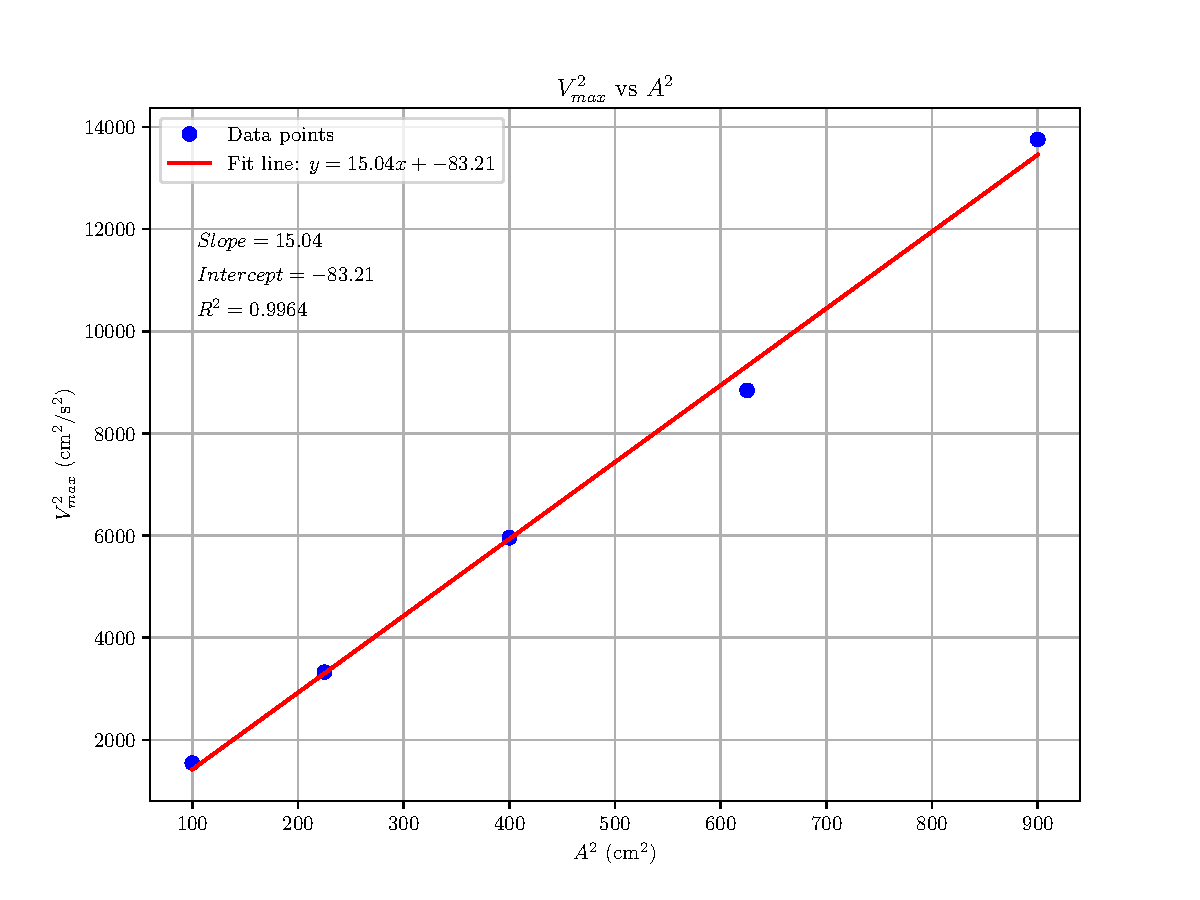
\includegraphics[width=0.8\textwidth]{./vmax2_vs_a2.pdf}
    \caption{平衡位置速度平方与振幅平方的关系}
    \label{fig:平衡位置速度平方与振幅平方的关系}
\end{figure}

根据上图可以得到，图像的斜率$k=15.04$,$\omega_0 = 3.878\text{s}^{-1}$，对应的周期为$1.6202\text{s}$。这一结果相对于实际测得的周期略微偏大，但和前面$v^2 - x^2$的实验结果相差不大，因此可以认为实验结果是合理的。

\subsection{不同U挡光片通过光电门所用的时间（AP距离为50cm）}

\begin{table}[H]
  \centering
	\begin{tabular}{|c|c|c|c|c|c|c|c|}
		\hline
		挡光片宽度（cm） & t1(ms) & t2(ms) & t3(ms) & t4(ms) & t5(ms) & t(ms)   & v           \\ \hline
		1(cm)     & 26.31  & 26.17  & 26.37  & 26.23  & 26.45  & 26.306  & 0.380141 \\ \hline
		3(cm)     & 77.98   & 77.84  & 77.71  & 78.01  & 78.36  & 77.980  & 0.384714 \\ \hline
		5(cm)     & 127.67 & 129.62 & 128.62 & 129.38 & 128.92 & 128.842 & 0.388072 \\ \hline
		10(cm)    & 252.48 & 250.98 & 252.03 & 252.65 & 251.13 & 251.854 & 0.397055 \\ \hline
	\end{tabular}
	\caption{不同U挡光片通过光电门所用的时间（AP距离为50cm）}
\end{table}

根据上述表格，绘制$t - v$的图像，结果如下：

\begin{figure}[H]
    \centering
    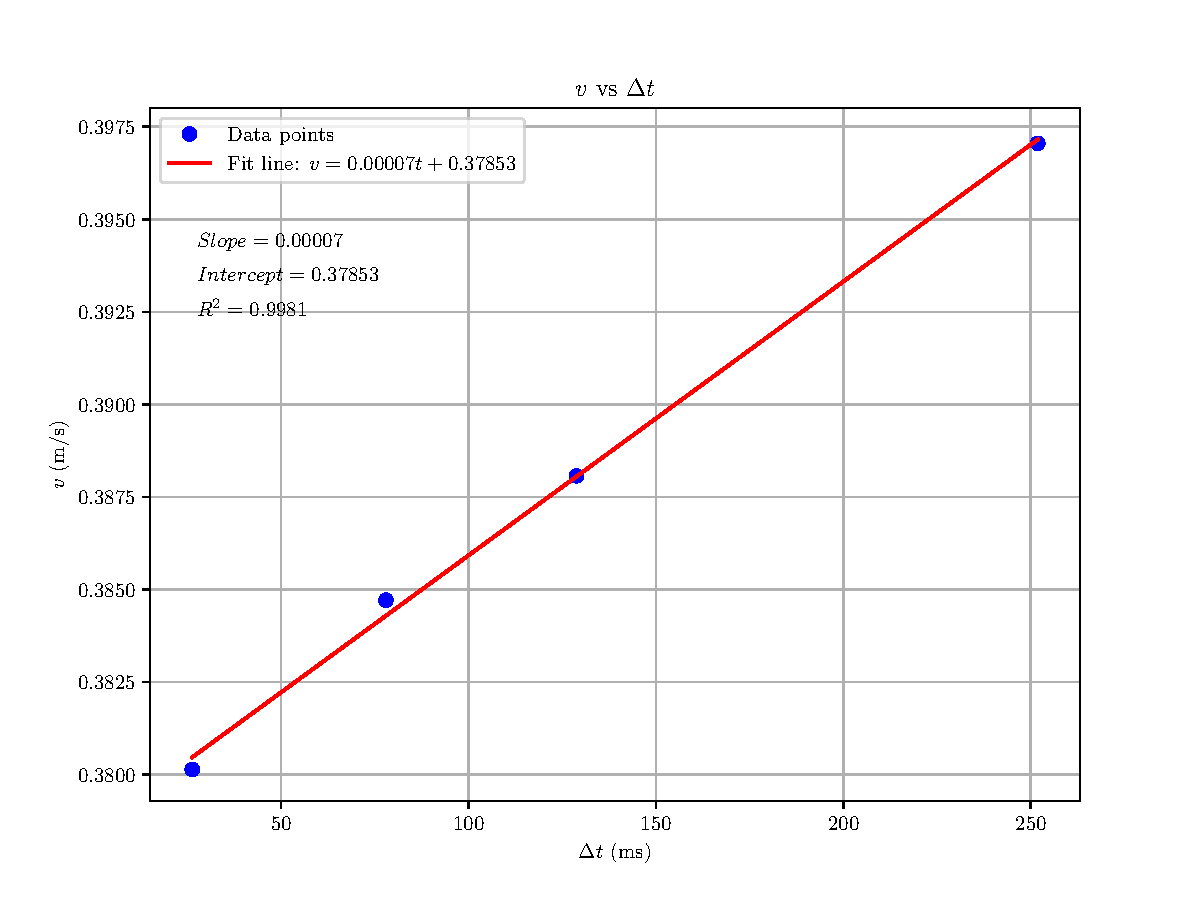
\includegraphics[width=0.8\textwidth]{./small_angle_and_50cm.pdf}
    \caption{不同U挡光片通过光电门所用的时间与速度的关系}
    \label{fig:不同U挡光片通过光电门所用的时间与速度的关系1}
\end{figure}

\subsection{不同U挡光片通过光电门所用的时间（AP距离为50cm），增大角度}

\begin{table}[H]
  \centering
	\begin{tabular}{|c|c|c|c|c|c|c|c|}
		\hline
		挡光片宽度（cm） & t1(ms) & t2(ms) & t3(ms) & t4(ms) & t5(ms) & t(ms)   & v           \\ \hline
		1(cm)     & 19.70  & 19.75  & 19.62  & 19.59  & 19.64  & 19.66  & 0.508647 \\ \hline
		3(cm)     & 58.26   & 58.20  & 58.15  & 57.96  & 58.09  & 58.132  & 0.516067 \\ \hline
		5(cm)     & 96.78 & 96.25 & 95.91 & 95.70 & 96.59 & 96.246 & 0.519502 \\ \hline
		10(cm)    & 187.78 & 187.39 & 188.38 & 188.05 & 187.98 & 187.916 & 0.532153 \\ \hline
	\end{tabular}
	\caption{不同U挡光片通过光电门所用的时间（AP距离为50cm），增大角度}
\end{table}

根据上述表格，绘制$t - v$的图像，结果如下：

\begin{figure}[H]
    \centering
    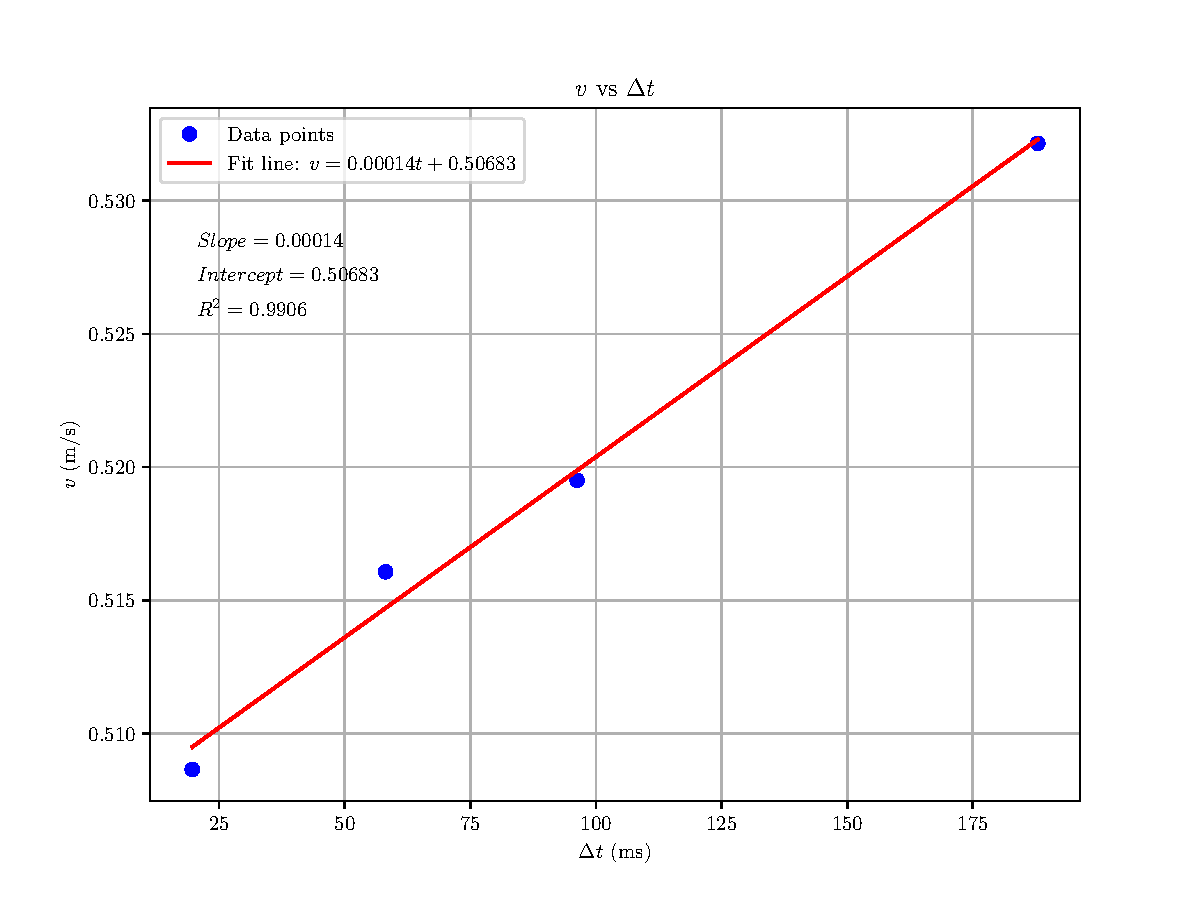
\includegraphics[width=0.8\textwidth]{./large_angle_and_50cm.pdf}
    \caption{不同U挡光片通过光电门所用的时间与速度的关系}
    \label{fig:不同U挡光片通过光电门所用的时间与速度的关系2}
\end{figure}

\subsection{不同U挡光片通过光电门所用的时间（AP距离为60cm）}

\begin{table}[H]
  \centering
	\begin{tabular}{|c|c|c|c|c|c|c|c|}
		\hline
		挡光片宽度（cm） & t1(ms) & t2(ms) & t3(ms) & t4(ms) & t5(ms) & t(ms)   & v           \\ \hline
		1(cm)     & 18.08  & 18.13  & 18.12  & 18.06  & 18.11  & 18.100  & 0.552486 \\ \hline
		3(cm)     & 53.67   & 53.65  & 53.65  & 53.64  & 53.69  & 53.660  & 0.559076 \\ \hline
		5(cm)     & 88.65 & 88.60 & 88.72 & 88.60 & 88.84 & 88.682 & 0.563812 \\ \hline
		10(cm)    & 174.69 & 174.18 & 174.18 & 174.17 & 173.89 & 174.222 & 0.573980 \\ \hline
	\end{tabular}
	\caption{不同U挡光片通过光电门所用的时间（AP距离为60cm）}
\end{table}

根据上述表格，绘制$t - v$的图像，结果如下：

\begin{figure}[H]
    \centering
    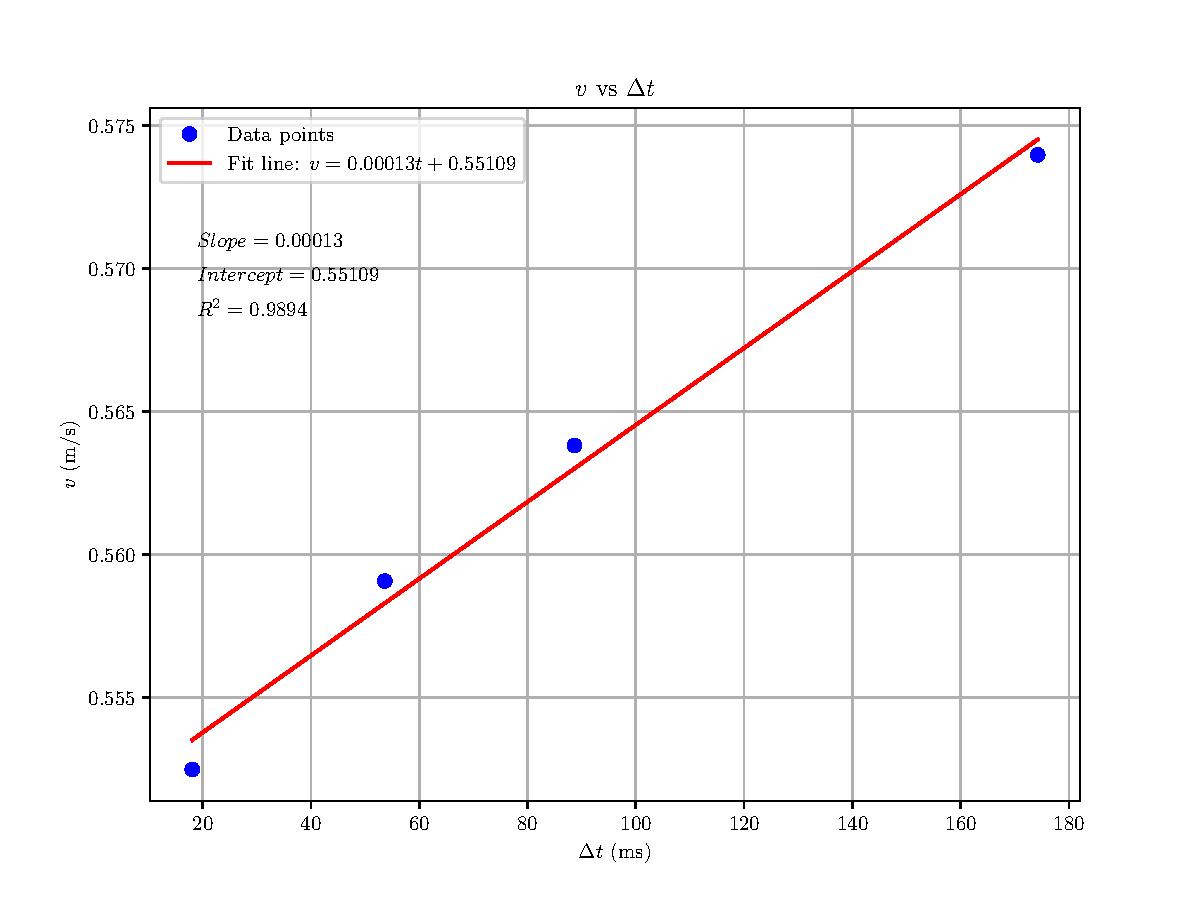
\includegraphics[width=0.8\textwidth]{./large_angle_and_60cm.pdf}
    \caption{不同U挡光片通过光电门所用的时间与速度的关系}
    \label{fig:不同U挡光片通过光电门所用的时间与速度的关系3}
\end{figure}

我们可以对以上实验结果的准确性进行检验。根据匀加速直线运动的速度公式：
\[
v = \sqrt{2 a L} = \sqrt{2 g L \sin\theta}
\]
其中，$g$ 为重力加速度，$L$ 为斜面长度，$\theta$ 为倾斜角。因此，应当有：
\[
v \propto \sqrt{L}
\]

比较图 \ref{fig:不同U挡光片通过光电门所用的时间与速度的关系3} 与图 \ref{fig:不同U挡光片通过光电门所用的时间与速度的关系2} 中的速度：
\[
\frac{0.552486}{0.508647} = 1.086, \quad \frac{0.559076}{0.516067} = 1.083, \quad \frac{0.563812}{0.519502} = 1.086, \quad \frac{0.573980}{0.532153} = 1.078
\]
而
\[
\sqrt{\frac{60}{50}} = 1.095
\]

可见，测量结果与理论预期基本一致。但是，四个测量结果的比值均比理论值小，这可能是由于实验中的摩擦力等因素导致的。

\section{总结与思考}

\subsection{思考题}
\begin{enumerate}
    \item 仔细观察，可以发现滑块的振幅是不断减小的，那么为什么还可以认为滑块是做简谐振动？实验中应如何尽量保证滑块做简谐振动？
    
        滑块的振幅虽然不断减小，但只要这种减小是缓慢且均匀的，它在前几个周期内的运动仍然可以近似地视为简谐振动。为了尽量保证滑块做简谐振动，我们应当进行以下操作：
        \begin{itemize}
            \item 开始实验前需要校准实验仪器，即气垫导轨需要调平。在相隔距离超过 80cm 的两点速度偏差不超过 $0.5 \%$ 时在进行实验，此时可以认为滑块的速度和振幅减小是非常缓慢的。
            \item 在实验过程中也需要注意，应当先开启气垫导轨，再放置滑块。这可以使导轨上形成一层均匀分布的气垫，减少气垫分布不均匀产生的水平方向的力对实验结果产生影响。
            \item 在实验过程中，我们应当尽可能的避免增加过多的骑码，以减少可能的摩擦，从而减慢振幅和速度的衰减速度。同时，也应当选择一个较大的初始振幅，如 40cm ，这样可以使初始的能量较大，速度的衰减较慢。此外，再测量时应当尽量选择靠前的几个周期的数据，这样可以减少振幅减小的影响。
            \item 在实验中，我们采用光电门和数字毫秒计测量周期和速度，能够提高实验精度。
        \end{itemize}

    \item 试说明弹簧的等效质量的物理意义，如不考虑弹簧的等效质量，则对实验结果有什么影响？
    
        弹簧的有效质量是指弹簧自身对振动系统总质量的贡献。需要考虑这部分质量的原因是，尽管弹簧本身的质量很小，但它并不是理想的轻质弹簧。弹簧自身的变形和回复作用也会对振动系统的整体行为有一定的贡献。为减小误差，把弹簧的动能动能平均化地视作一个质心位于滑块上，质量等于弹簧等效质量的物体运动的动能。事实上，我们将在下文证明，弹簧的有效质量是其自身质量的 $\frac{1}{3}$。经过这样的处理后，可以将弹簧理想化地看作轻弹簧。不考虑弹簧的有效质量会导致实验中算得的总机械能偏小。同时，也会导致计算出的周期偏短，因为实际振动系统的总质量比仅包含滑块的质量要大。这将导致对弹簧倔强系数$k$的估计值偏低。
        
    \item 测量周期时，光电门是否必须在平衡位置上？如不在平衡位置会产生什么不同的效果？
    
        在理想情况下，测量周期时光电门可以不位于平衡位置上，因为根据简谐运动的基本方程$x(t) = A \cos(\omega t + \varphi)$，可以看出，物体两次沿相同方向经过同一个$x_0$，时间间隔恰好为$T$。在实际测量中，滑块在平衡位置时的速度最大，因此挡光时间最短，导致测量周期的误差较小。而如果滑块距离平衡位置过远，振幅可能会迅速衰减，导致在测量进行到几组数据后，振幅减小至无法到达光电门的位置。因此，为了保证准确性，光电门最好放置在平衡位置或其附近。
        
    \item 气垫导轨如果不水平，是否能进行该实验？
    
        
如果气轨没有水平，那么运动方程满足 \( m\ddot{x} + kx + mg\sin\theta = 0 \)。 我们需要判断这一方程是否仍然简谐运动，就需要将其与简谐运动的标准形式进行比较。简谐运动的标准方程是 \( m\ddot{x} + kx = 0 \)，其中 \( m \) 是质量，\( k \) 是弹性常数，\( x \) 是位移，\( \ddot{x} \) 是加速度。从给定方程可以看出，\( m\ddot{x} + kx \) 部分与标准方程一致，但方程中还包含了一个额外的常数项 \( -mg\sin\theta \)，这个项与位移 \( x \) 无关。考虑到 \( \sin\theta \) 是一个常数，\( -mg\sin\theta \) 也是一个常数，因此它并不会改变系统的简谐性质，只是导致系统的平衡位置发生了偏移。为了恢复标准形式，我们可以定义新的坐标 \( x' = x + \frac{mg\sin\theta}{k} \)，此时方程变为 \( m\ddot{x'} + kx' = 0 \)，这是标准的简谐运动方程。因此，系统会围绕新的平衡位置 \( x' = -\frac{mg\sin\theta}{k} \) 进行简谐运动。因此，在倾斜状态下系统仍然做简谐运动，只是平衡位置发生了偏移。但在实际的实验中，当导轨倾斜时，每次更换砝码都会导致平衡位置的变化，这使得在测量不同质量滑块对振动周期的影响时，实验数据可能会受到干扰。此外，验证机械能守恒定律时，由于系统的重力势能变化无法准确测量，实验结果的准确性受到影响。特别是在导轨倾斜角度较大时，重力对运动的影响显著，可能会破坏简谐运动的假设。因此，为了确保实验的可靠性，导轨应保持水平状态，光电门最好设置在平衡位置附近，避免倾斜带来不必要的复杂性。

        
    \item 使用平板形挡光片和两个光电门，如何测量滑块通过倾斜气轨上某一点的瞬时速度？
    
       可以使用两个平板形挡光片拼接成U形挡光片，按照U形挡光片的操作测定瞬时速度。 
        
    \item 气垫导轨如果不水平，对瞬时速度的测定有什么影响？
    
        如果气垫导轨倾斜，可能会导致滑块发生一定程度的倾斜，且滑块的倾斜角度与气垫导轨的倾斜角度不同，从而增加滑块与气垫导轨之间的摩擦力。这种摩擦力会对滑块的运动产生影响，可能导致实验误差。然而，在实际实验中，气垫导轨的倾斜是刻意设计的，目的是为了使滑块获得初始速度，因此倾斜角度是实验设置的一部分，尽管它可能带来摩擦力，但也起到了提供初始速度的作用。
        
    \item 每次测量滑块和U型挡光片总质量不同是否对瞬时速度测定有影响？
    
理论上，滑块和U型挡光片的总质量不同不会对瞬时速度的测定产生影响。根据公式：

\[
v = \sqrt{2aL} = \sqrt{2gL \sin \theta}
\]

我们可以看到，速度 \(v\) 与质量无关，因此在理想情况下，质量的变化不应影响瞬时速度的测量。然而，在实际实验中，由于仪器设备的非理想性，质量的不同可能会引起导轨和滑块之间摩擦力的变化，从而对瞬时速度的测量产生一定的影响。这是因为摩擦力与质量相关，而摩擦力会影响滑块的运动状态，进而影响瞬时速度的准确测定。

\end{enumerate}

\subsection{实验心得}

\subsubsection{弹簧有效质量的推导}

下面我们证明弹簧的有效质量是其自身质量的 $\frac{1}{3}$，这需要考虑弹簧各部分的运动对总动能的贡献。

假设弹簧总质量为 $ m $，长度为 $ L $，弹性系数为 $ k $。弹簧的一端固定，另一端自由振动。

考虑弹簧的微元，取长度为 $ dx $ 的微小弹簧段，位于距离固定端 $ x $ 处。该微元的质量为：
$$
dm = \frac{m}{L} dx
$$

在简谐振动中，弹簧各处的位移与末端位移成比例，速度也成比例。微元处的速度为：
$$
v(x) = v_0 \left( \frac{x}{L} \right)
$$
其中，$ v_0 $ 为弹簧末端的速度。

微元的动能为：
$$
dT = \frac{1}{2} dm \cdot v(x)^2 = \frac{1}{2} \left( \frac{m}{L} dx \right) \left( v_0 \frac{x}{L} \right)^2
$$

将微元的动能在整个弹簧上积分：
$$
T = \int_0^L dT = \int_0^L \frac{1}{2} \left( \frac{m}{L} \right) \left( v_0 \frac{x}{L} \right)^2 dx
$$

执行积分：
$$
T = \frac{1}{2} \left( \frac{m}{L} \right) v_0^2 \int_0^L \left( \frac{x}{L} \right)^2 dx
$$
$$
= \frac{1}{2} \left( \frac{m}{L} \right) v_0^2 \int_0^L \frac{x^2}{L^2} dx
$$
$$
= \frac{1}{2} \left( \frac{m}{L} \right) v_0^2 \frac{1}{L^2} \int_0^L x^2 dx
$$
$$
= \frac{1}{2} \left( \frac{m}{L} \right) v_0^2 \frac{1}{L^2} \left[ \frac{x^3}{3} \right]_0^L
$$
$$
= \frac{1}{2} \left( \frac{m}{L} \right) v_0^2 \frac{1}{L^2} \left( \frac{L^3}{3} \right)
$$
$$
= \frac{1}{2} \left( \frac{m}{L} \right) v_0^2 \frac{L^3}{3L^2}
$$
$$
= \frac{1}{2} \left( \frac{m}{L} \right) v_0^2 \frac{L}{3}
$$
$$
= \frac{1}{2} \left( \frac{m}{3} \right) v_0^2
$$

将弹簧的总动能等效为集中质量 $ m_{\text{eff}} $ 的动能：
$$
T = \frac{1}{2} m_{\text{eff}} v_0^2
$$

比较两者得：
$$
\frac{1}{2} \left( \frac{m}{3} \right) v_0^2 = \frac{1}{2} m_{\text{eff}} v_0^2
$$

因此：
$$
m_{\text{eff}} = \frac{m}{3}
$$

\subsubsection{关于测得弹簧有效质量为负值的再讨论}
在前文中测得，弹簧的有效质量为负值，这是非常不合理的。为了避免数据过少，拟合直线的误差对实验结果造成影响，我们再使用逐差法来求出弹簧的有效质量 \( m_0 \)。具体步骤如下：

\begin{table}[h]
  \centering
  \begin{tabular}{|c|c|c|}
    \hline
    组别 & 平均周期 \( T \)（ms） & 质量 \( m \)（g） \\
    \hline
    1 & 1570.844 & 217.12 \\
    \hline
    2 & 1614.778 & 229.48 \\
    \hline
    3 & 1657.335 & 241.95 \\
    \hline
    4 & 1698.388 & 251.69 \\
    \hline
    5 & 1739.027 & 264.23 \\
    \hline
  \end{tabular}
  \caption{不同质量下的振动周期}
\end{table}

\textbf{步骤一：将周期从毫秒转换为秒} \\
\[
\begin{aligned}
T_1 &= 1570.844 \, \text{ms} = 1.570844 \, \text{s} \\
T_2 &= 1614.778 \, \text{ms} = 1.614778 \, \text{s} \\
T_3 &= 1657.335 \, \text{ms} = 1.657335 \, \text{s} \\
T_4 &= 1698.388 \, \text{ms} = 1.698388 \, \text{s} \\
T_5 &= 1739.027 \, \text{ms} = 1.739027 \, \text{s} \\
\end{aligned}
\]

\textbf{步骤二：计算周期的平方 \( T^2 \)} \\
\[
\begin{aligned}
T_1^2 &= (1.570844)^2 \approx 2.467 \, \text{s}^2 \\
T_2^2 &= (1.614778)^2 \approx 2.606 \, \text{s}^2 \\
T_3^2 &= (1.657335)^2 \approx 2.754 \, \text{s}^2 \\
T_4^2 &= (1.698388)^2 \approx 2.894 \, \text{s}^2 \\
T_5^2 &= (1.739027)^2 \approx 3.022 \, \text{s}^2 \\
\end{aligned}
\]

\textbf{步骤三：计算差分 \( \Delta T^2 \) 和 \( \Delta m \)} \\
\[
\begin{aligned}
\Delta T^2_{1} &= T_2^2 - T_1^2 = 2.606 - 2.467 = 0.139 \, \text{s}^2 \\
\Delta T^2_{2} &= T_3^2 - T_2^2 = 2.754 - 2.606 = 0.148 \, \text{s}^2 \\
\Delta T^2_{3} &= T_4^2 - T_3^2 = 2.894 - 2.754 = 0.140 \, \text{s}^2 \\
\Delta T^2_{4} &= T_5^2 - T_4^2 = 3.022 - 2.894 = 0.128 \, \text{s}^2 \\
\end{aligned}
\]

\[
\begin{aligned}
\Delta m_{1} &= m_2 - m_1 = 229.48 - 217.12 = 12.36 \, \text{g} \\
\Delta m_{2} &= m_3 - m_2 = 241.95 - 229.48 = 12.47 \, \text{g} \\
\Delta m_{3} &= m_4 - m_3 = 251.69 - 241.95 = 9.74 \, \text{g} \\
\Delta m_{4} &= m_5 - m_4 = 264.23 - 251.69 = 12.54 \, \text{g} \\
\end{aligned}
\]

\textbf{步骤四：计算斜率 \( k \)} \\
根据理论公式：
\[
T^2 = \frac{4\pi^2}{k}(m + m_0)
\]
差分后：
\[
\Delta T^2 = \frac{4\pi^2}{k} \Delta m
\]
因此，斜率 \( k \) 可表示为：
\[
k = \frac{4\pi^2 \Delta m}{\Delta T^2}
\]

计算每组差分得到的斜率：
\[
\begin{aligned}
k_1 &= \frac{4\pi^2 \times 12.36}{0.139} \approx \frac{39.478 \times 12.36}{0.139 \cdot 1000} \approx 3.51845 \, \text{N/m} \\
k_2 &= \frac{4\pi^2 \times 12.47}{0.148} \approx \frac{39.478 \times 12.47}{0.148 \cdot 1000} \approx 3.33345 \, \text{N/m} \\
k_3 &= \frac{4\pi^2 \times 9.74}{0.140} \approx \frac{39.478 \times 9.74}{0.140 \cdot 1000} \approx 2.75693 \, \text{N/m} \\
k_4 &= \frac{4\pi^2 \times 12.54}{0.128} \approx \frac{39.478 \times 12.54}{0.128 \cdot 1000} \approx 3.87025 \, \text{N/m} \\
\end{aligned}
\]

取斜率的平均值：
\[
k_{\text{平均}} = \frac{3.51845 + 3.33345 + 2.75693 + 3.87025}{4} \approx 3.37402 \, \text{N/m}
\]

在这里，我们看到，第三个数据点明显偏离其他数据点，这可能是由于实验误差导致的。因此，我们可以考虑排除第三个数据点，重新计算斜率的平均值：
\[
k_{\text{平均}} = \frac{3.51845 + 3.33345 + 3.87025}{3} \approx 3.57472 \, \text{N/m}
\]

\textbf{步骤五：计算弹簧的有效质量 \( m_0 \)} \\
利用第一组数据来求解截距，从而得到 \( m_0 \)。

根据公式：
\[
T^2 = \frac{4\pi^2}{k}(m + m_0)
\]
可以重写为：
\[
m_0 = \frac{k T^2}{4\pi^2} - m
\]

使用第一组数据：
\[
m_0 = \frac{3.57472 \times 2.467}{39.478} - 0.21712 \approx  6.49 \, \text{g}
\]

\textbf{计算结果分析} \\
计算得到的弹簧有效质量 \( m_0 \approx 6.49 \, \text{g} \) ，这在物理上是合理的，并且与上一部分的推导相吻合。这说明，实验的误差是第三组数据，即第三个数据点或第四个数据点的测量偏差导致的。为了进一步验证这一结果，可以考虑重复实验，增加实验次数，取更多数据点以减小误差。

\end{document}

% VScode 常用快捷键：

% F2:                       变量重命名
% Ctrl + Enter:             行中换行
% Alt + up/down:            上下移行
% 鼠标中键 + 移动:           快速多光标
% Shift + Alt + up/down:    上下复制
% Ctrl + left/right:        左右跳单词
% Ctrl + Backspace/Delete:  左右删单词    
% Shift + Delete:           删除此行
% Ctrl + J:                 打开 VScode 下栏(输出栏)
% Ctrl + B:                 打开 VScode 左栏(目录栏)
% Ctrl + `:                 打开 VScode 终端栏
% Ctrl + 0:                 定位文件
% Ctrl + Tab:               切换已打开的文件(切标签)
% Ctrl + Shift + P:         打开全局命令(设置)

% Latex 常用快捷键：

% Ctrl + Alt + J:           由代码定位到PDF


